\documentclass[journal,twoside,web]{ieeecolor}
\usepackage{generic}
\usepackage{cite}
\usepackage{amsmath,amssymb,amsfonts}
\usepackage{algorithmic}
\usepackage{graphicx}
\usepackage{tikz}
\usetikzlibrary{arrows.meta,positioning}
\usepackage{booktabs}
\usepackage{algorithm,algorithmic}
\usepackage{hyperref}
\hypersetup{hidelinks}
\usepackage{textcomp}
\def\BibTeX{{\rm B\kern-.05em{\sc i\kern-.025em b}\kern-.08em
    T\kern-.1667em\lower.7ex\hbox{E}\kern-.125emX}}
\markboth{\hskip25pc IEEE TRANSACTIONS AND JOURNALS TEMPLATE}
{Author \MakeLowercase{\textit{et al.}}: Title}
\begin{document}
\title{Which Adaptation Strategy for a New Task? A Controlled Study of\\Parameter-Efficient Continual Learning on 3D Brain MRI}

% ---------------------------------------------------------------------------
% REVISION NOTE (2026-09-12). All numbers in this file come from the corrected
% protocol (PROTOCOL_AUDIT.md): subject-grouped held-out test set, whole-volume
% sliding-window inference (overlap 0.25), per-case metrics, real IXI ages,
% unlabelled BraTS cases excluded. Values are mean +/- SD over seeds 42-44 from
% outputs/benchmark_v2/n32/. The pre-audit manuscript is preserved as
% main_v1_original_2026-09-05.tex.
% ---------------------------------------------------------------------------

\author{Chi-Sheng Chen$^{1}$,
Xinyu Zhang$^{2}$,
En-Jui Kuo$^{5}$,
Rong Fu$^{2}$,
Qiuzhe Xie$^{3}$,
and Fan Zhang$^{4}$
\thanks{$^{1}$Beth Israel Deaconess Medical Center \& Harvard Medical School, Boston, MA 02115 USA.}
\thanks{$^{2}$Luddy School of Informatics, Computing, and Engineering, Indiana University Bloomington, Bloomington, IN 47405 USA.}
\thanks{$^{3}$Institute of Electronics Engineering, National Taiwan University, 106319, Taiwan.}
\thanks{$^{4}$Department of Mathematics, Boise State University, Boise, ID 83702 USA.}
\thanks{$^{5}$Department of Electrophysics, National Yang Ming Chiao Tung University, 30010, Taiwan.}}

\maketitle

\begin{abstract}
A department that adds a new analysis task to an existing imaging workflow typically has a few dozen annotated cases, no access to the data behind the tasks already deployed, and a model it cannot afford to retrain or to store many copies of. Which adaptation strategy should it choose? We answer this empirically for 3D brain MRI, comparing ten strategies---low-rank adaptation (LoRA), bias-only tuning, linear probing, full fine-tuning, and the standard continual-learning remedies EWC, LwF and experience replay---across five tasks spanning three output types at 32 labeled volumes each: glioma segmentation (BraTS 2023), stroke-lesion segmentation (ISLES 2022), hippocampus segmentation (MSD), brain-age regression and sex classification (IXI), under a subject-grouped held-out protocol with whole-volume inference and three random seeds. The choice turns on one property of the new task: whether it inherits a large task-specific head. All three segmentation tasks do, and there training that decoder directly is best, beating LoRA by a stable 0.011--0.015 Dice---but at 8.45\,MB of trainable parameters and 32\,MB of per-task storage against LoRA's 93.8\,K and 366\,KB. Neither global task does, and there LoRA is the only frozen-backbone strategy that works at all: brain-age MAE $10.22\pm0.82$\,yr ($R^2{=}0.40$) against a 14.4\,yr constant baseline and sex AUC $0.876\pm0.079$, each beating full fine-tuning of 14\,M parameters, while linear probing and bias-only tuning return a constant output despite their frozen features ranking subjects well above chance. We also report three findings that bear directly on practice: freezing shared weights is the only reliable route to zero forgetting, as EWC, LwF and replay each forget \emph{more} than unregularised fine-tuning; a pretrained checkpoint should be validated rather than assumed to transfer, since ours is no better than random initialisation ($-0.009$ Dice, $p{=}3{\times}10^{-9}$); and an evaluation protocol that scores random crops on the model-selection split inflates results enough to reverse conclusions. Code, splits, per-case predictions and the protocol are released.
\end{abstract}

\begin{IEEEkeywords}
Clinical model deployment \and Few-shot learning \and Continual learning \and Parameter-efficient fine-tuning \and LoRA \and 3D brain MRI.
\end{IEEEkeywords}

\section{Introduction}
\label{sec:introduction}

\IEEEPARstart{A}{} hospital imaging service rarely deploys one model and stops. A department running automated tumour segmentation may later want stroke-lesion delineation, then a quantitative marker such as brain age; each capability arrives with a small batch of newly annotated cases, months apart, and typically without access to the data behind the capabilities already in service---retained either not at all, or under governance that makes reuse impractical~\cite{fomo2025,baseline}. The engineering question this poses is concrete: given a frozen model that already works, 32 annotated volumes, and no prior-task data, which adaptation strategy should be used, and what does each cost to run and to store?

The options span four orders of magnitude of trainable parameters. At one end, full fine-tuning updates everything and is the usual default; it also overwrites the representation the earlier tasks depend on, causing \emph{catastrophic forgetting}~\cite{kirkpatrick2017,mccloskey1989catastrophic}, and requires a separate copy of the whole network per task. Regularisation- and distillation-based remedies such as EWC~\cite{kirkpatrick2017} and LwF~\cite{li2017lwf} aim to soften that at the cost of tuning effort. At the other end, the backbone can be \emph{frozen} and only small task-specific modules trained: a linear probe over frozen features, bias-only tuning~\cite{bitfit}, or low-rank adaptation (LoRA)~\cite{hu2022lora,hu2024computational}, which injects trainable low-rank matrices while leaving the original weights untouched. Freezing has an operational attraction beyond compute: because prior-task parameters are never modified, prior-task behaviour cannot change, and because nothing is replayed, no earlier patient data need be retained---a property that matters where retention is governed by HIPAA or GDPR.

Which of these to choose is usually settled by habit rather than evidence, and the evidence that exists is fragmented across single tasks and inconsistent protocols. We therefore ran the comparison directly: ten strategies, five tasks spanning segmentation, regression and classification, four public cohorts, three seeds, one protocol.

The answer turns out to be neither ``adapters are efficient'' nor ``fine-tuning is better'', but conditional on a property of the new task that is knowable in advance---whether it inherits a large task-specific head---and the two cases point in opposite directions.

Reaching that answer required first settling how it is measured. The evaluation pipeline we initially built, following what is common in this literature, reported on the same split used for model selection, scored a single random $64^3$ crop per case, pooled voxels across cases into one Dice, and let longitudinal timepoints of one patient span training and test. Each of these inflates results, and together they were enough to reverse conclusions: under that pipeline LoRA appeared to underperform linear probing on segmentation by 0.19 Dice, where the true gap is 0.012. We replaced it with subject-grouped train/validation/test splits, whole-volume sliding-window inference, and per-case Dice and 95th-percentile Hausdorff distance (HD95), and report every number below under that protocol. Section~\ref{sec:protocol} specifies it; we release it with the code because the same failure modes are easy to reproduce accidentally.

Our findings and contributions are:
\begin{itemize}
\item \textbf{Where a task has no large head, LoRA is necessary, not merely economical---shown twice.} On whole-head input, brain age reaches MAE $10.22\pm0.82$\,yr ($R^2=0.40$) against a constant baseline of 14.4, and sex classification AUC $0.876\pm0.079$; both beat full fine-tuning of every parameter (by 1.98\,yr and by 0.11 per-case accuracy respectively) with 56K trainable. Frozen-encoder linear probing and BitFit collapse to a constant output on both, despite the frozen features carrying usable signal (linear-probe sex AUC 0.717, well above chance): the information is present but unusable without moving the representation.
\item \textbf{Where a large task head already exists, LoRA gives up a small, stable margin for 90$\times$ fewer parameters---shown three times.} Across glioma, stroke-lesion and hippocampus segmentation, full-decoder linear probing leads by $0.012$, $0.015$ and $0.011$ Dice respectively while training 8.45M parameters against 93.8K; at 64 shots the two are equal.
\item \textbf{A 66-parameter configuration detail dominates.} Leaving the segmentation output projection frozen, as ``frozen backbone'' naively implies, costs $0.217$ Dice ($p<10^{-130}$) and triples seed variance.
\item \textbf{Forgetting-free is shared, and the standard remedies do not deliver it.} Adapter isolation and frozen-encoder probing both have BWT exactly zero over a three-task sequence in which full fine-tuning loses $0.55$ Dice; EWC, LwF and replay all forget \emph{more} than unregularised fine-tuning ($-0.39$, $-0.56$, $-0.37$ vs.\ $-0.33$).
\item \textbf{A negative result on pretraining.} The pretrained checkpoint is not better than random initialisation for the frozen backbone ($-0.009$ Dice, $p=3{\times}10^{-9}$). We therefore claim parameter-efficient adaptation, not transfer.
\item \textbf{A corrected evaluation protocol and code}, with tests that guard the label-handling and split-leakage failures we encountered---including one that silently zeroed every mask of a single-channel dataset while validation reported a perfect score.
\end{itemize}


\section{Related Work}
\label{sec:related}

\subsection{Foundation Models for Medical Imaging}

Large-scale pretrained models have transformed medical image analysis. The FOMO initiative~\cite{fomo2025} provides 3D foundation models pretrained on diverse medical imaging datasets via masked autoencoding objectives, yielding general-purpose representations for downstream adaptation. UNETR~\cite{unetr} introduced Vision Transformers into 3D medical segmentation by replacing CNN encoders with self-attention, demonstrating strong performance on multi-organ and brain tumor segmentation. More recently, SAM-Med3D~\cite{sammed3d} extended the Segment Anything paradigm to volumetric data, and domain-specific foundation models have emerged for pathology~\cite{chen2024towards} and radiology. These models share a common deployment challenge: adapting to multiple downstream tasks efficiently while preserving the pretrained representations, particularly when labeled data is scarce.

\subsection{Continual Learning in Medical Imaging}

Continual learning addresses the problem of sequentially learning new tasks without forgetting previously acquired knowledge~\cite{mccloskey1989catastrophic}. Classical approaches fall into three categories: (i)~\emph{regularization-based} methods such as EWC~\cite{kirkpatrick2017} and Synaptic Intelligence~\cite{zenke2017continual}, which penalize changes to important parameters; (ii)~\emph{replay-based} methods such as iCaRL~\cite{rebuffi2017icarl}, which store or generate exemplars from prior tasks; and (iii)~\emph{distillation-based} methods such as LwF~\cite{li2017lwf}, which use the previous model's outputs as soft targets. In medical imaging, continual learning has been explored primarily for class-incremental segmentation: LifeLonger~\cite{derakhshani2022lifelonger} benchmarks continual disease classification across dermatology datasets, while Lifelong nnU-Net~\cite{gonzalez2023lifelong} standardizes continual organ segmentation. However, most prior work considers \emph{class-incremental} settings with homogeneous outputs (e.g., adding new organ classes). Our work addresses \emph{task-incremental} continual learning across \emph{heterogeneous} output types---segmentation, regression and classification---which presents distinct challenges since the task heads and loss functions differ fundamentally, and, as Section~\ref{sec:res_replicate} shows, the right adaptation strategy differs with them.

\subsection{Parameter-Efficient Fine-Tuning}

Parameter-efficient fine-tuning (PEFT) methods adapt large pretrained models by training only a small subset of parameters. LoRA~\cite{hu2022lora} injects trainable low-rank decompositions into weight matrices, achieving competitive performance with full fine-tuning at a fraction of the parameter cost. Alternative PEFT approaches include Adapters~\cite{houlsby2019}, which insert bottleneck modules between layers; Prefix-Tuning~\cite{prefix_tuning}, which prepends learnable tokens to the input; and BitFit~\cite{bitfit}, which tunes only bias terms. In the context of continual learning, PEFT methods offer a natural mechanism for task isolation: PackNet~\cite{packnet} iteratively prunes and freezes network capacity per task, while Piggyback~\cite{piggyback} learns binary masks over a shared backbone. Our approach is most closely related to adapter-isolation strategies but applies LoRA's low-rank structure to 3D convolutions, which is directly compatible with pretrained U-Net architectures. A recurring detail in the PEFT literature, and the one that turns out to matter most here, is that the task-specific output layer is always trained alongside the low-rank updates; a pretrained projection cannot be expected to map onto a new label space.


\section{Method}
\label{sec:method}

\subsection{Problem Formulation}
\label{sec:problem}

We consider continual learning with sequential task arrival. Let $f_\theta$ denote a pretrained 3D U-Net backbone (frozen) and $\mathcal{T}_1, \mathcal{T}_2, \ldots, \mathcal{T}_K$ a sequence of tasks. For each task $k$, we have access to only $N_k$ labeled few-shot samples ($N_k = 32$ throughout) drawn from task-specific distribution $\mathcal{D}_k = \{(x_i^{(k)}, y_i^{(k)})\}_{i=1}^{N_k}$. We assume \emph{no replay}: when training on $\mathcal{T}_k$, we cannot access data from $\mathcal{T}_{<k}$. The optimization objective for task $k$ is:
\begin{equation}
\min_{\phi_k, h_k} \; \frac{1}{N_k} \sum_{i=1}^{N_k} \mathcal{L}_k \bigl( h_k(f_\theta(x_i^{(k)}; \phi_k)),\; y_i^{(k)} \bigr)
\label{eq:objective}
\end{equation}
where $\phi_k$ denotes the LoRA adapter parameters for task $k$, $h_k$ the task-specific head, and $\mathcal{L}_k$ the task loss. Crucially, $\theta$ remains frozen throughout; only $\phi_k$ and $h_k$ are optimized. The goal is to learn $\{\phi_k, h_k\}_{k=1}^K$ such that performance on all seen tasks remains high after training on $\mathcal{T}_K$.

We evaluate two tasks: (1) tumor segmentation (3D binary mask) and (2) brain age estimation (regression). Each task has modality-specific inputs (BraTS: T2w, T2-FLAIR, T1c; IXI: T1, T2) and a distinct output head $h_k$. Because the modality counts differ, the first convolution of the encoder cannot be shared and is task-specific; all remaining encoder weights (39 of 40 tensors) are shared and frozen.

Figure~\ref{fig:framework} illustrates the overall pipeline: a frozen pretrained backbone, task-specific LoRA adapters, and task heads. At inference for task $k$, we use backbone $f_\theta$ + adapter $\phi_k$ + head $h_k$; prior adapters and the backbone remain frozen. Task identity is assumed known at inference.

\begin{figure*}[t]
\centering
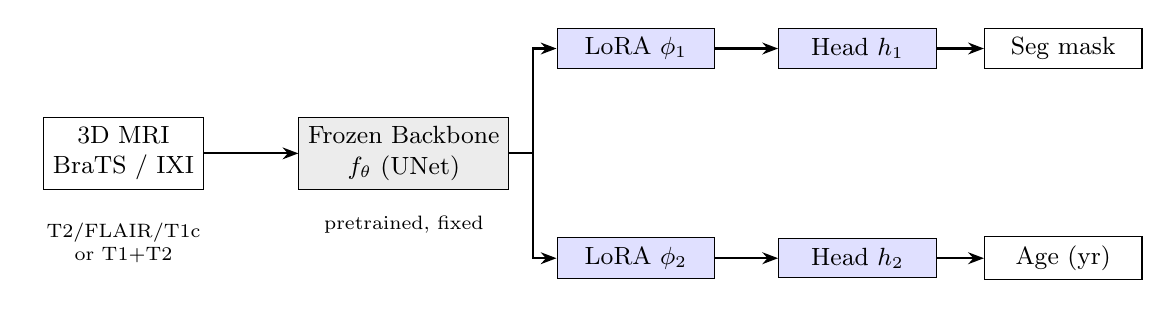
\begin{tikzpicture}[
  node distance=0.5cm and 0.8cm,
  box/.style={draw, minimum width=2cm, minimum height=0.5cm, align=center, font=\small},
  bigbox/.style={draw, minimum width=2.2cm, minimum height=0.7cm, align=center, font=\small},
  frozen/.style={fill=gray!15, box},
  trainable/.style={fill=blue!12, box},
  arrow/.style={-{Stealth[length=2mm]}, thick}
]
  \node[box] (input) {3D MRI\\BraTS / IXI};
  \node[below=0.3cm of input, font=\scriptsize, text width=2.2cm, align=center] {T2/FLAIR/T1c or T1+T2};
  \node[bigbox, frozen, right=1.2cm of input] (backbone) {Frozen Backbone\\$f_\theta$ (UNet)};
  \node[below=0.2cm of backbone, font=\scriptsize] {pretrained, fixed};
  \node[box, trainable, above right=0.6cm and 0.6cm of backbone] (lora1) {LoRA $\phi_1$};
  \node[box, trainable, below right=0.6cm and 0.6cm of backbone] (lora2) {LoRA $\phi_2$};
  \node[box, trainable, right=0.8cm of lora1] (head1) {Head $h_1$};
  \node[box, trainable, right=0.8cm of lora2] (head2) {Head $h_2$};
  \node[box, right=0.6cm of head1] (out1) {Seg mask};
  \node[box, right=0.6cm of head2] (out2) {Age (yr)};
  \draw[arrow] (input) -- (backbone);
  \draw[arrow] (backbone.east) -- ++(0.3,0) |- (lora1.west);
  \draw[arrow] (backbone.east) -- ++(0.3,0) |- (lora2.west);
  \draw[arrow] (lora1) -- (head1);
  \draw[arrow] (lora2) -- (head2);
  \draw[arrow] (head1) -- (out1);
  \draw[arrow] (head2) -- (out2);
\end{tikzpicture}
\caption{Framework: frozen pretrained backbone $f_\theta$ with task-specific LoRA adapters $\phi_k$ and heads $h_k$. Gray = frozen; blue = trainable per task. At inference for T1 (resp.\ T2): backbone + $\phi_1$ + $h_1$ (resp.\ $\phi_2$ + $h_2$). For segmentation, $h_1$ is the $1{\times}1{\times}1$ output projection of the U-Net decoder (66 parameters); leaving it frozen is the single largest source of error we observed (Sec.~\ref{sec:res_head}).}
\label{fig:framework}
\end{figure*}

\subsection{LoRA for 3D Convolutions}
\label{sec:lora}

Low-Rank Adaptation (LoRA)~\cite{hu2022lora} injects trainable low-rank matrices into a frozen weight matrix $W \in \mathbb{R}^{d \times k}$:
\begin{equation}
W' = W + \Delta W, \quad \Delta W = \frac{\alpha}{r} B \cdot A, \quad A \in \mathbb{R}^{r \times k}, \; B \in \mathbb{R}^{d \times r}
\label{eq:lora}
\end{equation}
with rank $r \ll \min(d,k)$ and scaling factor $\alpha$. Only $A$ and $B$ are trained; $W$ stays frozen. The scaling ratio $\alpha/r$ controls the magnitude of the low-rank perturbation relative to the pretrained weights.

For 3D convolutions in a U-Net, we apply LoRA via parallel $1\times1\times1$ convolutions acting on the channel dimension:
\begin{equation}
\text{Conv3d}'(x) = \text{Conv3d}(x; W) + \frac{\alpha}{r} \, \text{Conv1}(x; B) \circ \text{Conv1}(x; A)
\label{eq:lora3d}
\end{equation}
where Conv1 denotes $1\times1\times1$ convolution, $A \in \mathbb{R}^{r \times C_{\text{in}}}$ projects to rank-$r$ space, and $B \in \mathbb{R}^{C_{\text{out}} \times r}$ projects back. This formulation is memory-efficient and compatible with standard Conv3d layers~\cite{peft}.

We use $\alpha=16$, evaluate $r \in \{4, 8, 16\}$ (Sec.~\ref{sec:res_rank}) and report $r=16$, and target every Conv3d in both encoder and decoder for segmentation; encoder-only suffices for regression. For a single Conv3d layer with input channels $C_{\text{in}}$ and output channels $C_{\text{out}}$, the number of LoRA parameters is:
\begin{equation}
|\phi_{\text{layer}}| = r \cdot (C_{\text{in}} + C_{\text{out}})
\label{eq:param_count}
\end{equation}
which is substantially smaller than the original $C_{\text{out}} \times C_{\text{in}} \times D \times H \times W$ parameters. Summed over all targeted layers at $r=16$, the adapter for segmentation has 93,810 parameters against a 22.63M-parameter U-Net (0.41\%), and the adapter for regression has 55,841 parameters against the 14.16M-parameter encoder-plus-head (0.39\%); at $r=8$ the counts are 46,872 and 28,177.

\subsection{Continual Learning via Adapter Isolation}
\label{sec:continual}

Each task $k$ receives a \emph{dedicated LoRA adapter} $\phi_k$. The full training and inference procedure is summarized in Algorithm~\ref{alg:continual}. The trainable parameter set for task $k$ is strictly disjoint from all other tasks:
\begin{equation}
\Phi_k = \{\phi_k, h_k\}, \quad \Phi_i \cap \Phi_j = \emptyset \;\; \forall \, i \neq j
\label{eq:disjoint}
\end{equation}
Because $\theta$ and $\{\Phi_{<k}\}$ are frozen when optimizing $\Phi_k$, the performance of any prior task $j < k$ is invariant to training on $\mathcal{T}_k$. Formally, let $R_{t,j}$ denote the performance of task $j$ after training up to task $t$. Then:
\begin{equation}
R_{t,j} = R_{j,j} \quad \forall \, t \geq j \implies \text{BWT}_j = R_{K,j} - R_{j,j} = 0
\label{eq:bwt_zero}
\end{equation}
This zero-forgetting property holds \emph{by construction}, without regularization or replay. It is not, however, unique to adapters: any scheme that leaves shared weights untouched---including linear probing on a frozen encoder---satisfies Eq.~\eqref{eq:bwt_zero} equally. What distinguishes the schemes is how many parameters they must train to reach a given accuracy, which is what Section~\ref{sec:results} measures. The total model storage after $K$ tasks is:
\begin{equation}
\text{Storage} = |\theta| + \sum_{k=1}^{K} (|\phi_k| + |h_k|)
\label{eq:storage}
\end{equation}
which grows linearly in $K$ with a small per-task overhead since $|\phi_k| \ll |\theta|$.

\begin{algorithm}[t]
\caption{Continual Learning via LoRA Adapter Isolation}
\label{alg:continual}
\begin{algorithmic}[1]
\REQUIRE Pretrained backbone $f_\theta$; task sequence $\mathcal{T}_1, \ldots, \mathcal{T}_K$; subject-grouped train/val/test splits per task; LoRA rank $r$; epochs $E$
\ENSURE Trained adapters $\{\phi_k\}_{k=1}^K$ and heads $\{h_k\}_{k=1}^K$
\STATE Freeze all parameters of $f_\theta$
\FOR{$k = 1$ \TO $K$}
    \STATE Initialize LoRA adapter $\phi_k$ with rank $r$ (Kaiming $A$, zero $B$)
    \STATE Initialize task head $h_k$ (output projection for segmentation; pooled regressor for regression); mark trainable
    \IF{$k > 1$}
        \STATE Freeze all previous adapters $\phi_1, \ldots, \phi_{k-1}$ and heads $h_1, \ldots, h_{k-1}$
    \ENDIF
    \FOR{epoch $= 1$ \TO $E$}
        \FOR{each mini-batch $(x, y) \in \mathcal{D}_k^{\text{train}}$}
            \STATE $\hat{y} \leftarrow h_k(f_\theta(x; \phi_k))$
            \STATE Update $\phi_k, h_k$ on $\mathcal{L}_k(\hat{y}, y)$ with AdamW
        \ENDFOR
        \STATE Score $\mathcal{D}_k^{\text{val}}$ (deterministic centre crop); keep the best epoch
    \ENDFOR
    \STATE Score the kept checkpoint once on $\mathcal{D}_k^{\text{test}}$ with whole-volume inference
\ENDFOR
\end{algorithmic}
\end{algorithm}

\subsection{Task Heads and Losses}
\label{sec:heads}

\textbf{Task 1 (Segmentation).} The full U-Net decoder produces a voxel-wise two-class prediction. LoRA is applied to every Conv3d in encoder and decoder. The head $h_1$ is the decoder's final $1{\times}1{\times}1$ projection from 32 channels to the 2 output classes (66 parameters), which is trained from its pretrained initialization. We stress this because a natural but wrong reading of ``frozen backbone'' is to freeze this layer too; Section~\ref{sec:res_head} quantifies the consequence. The training loss is cross-entropy plus soft Dice on the foreground probability:
\begin{equation}
\mathcal{L}_{\text{seg}} = \text{CE}(p, g) + 1 - \frac{2 \sum_i p_i g_i + \epsilon}{\sum_i p_i + \sum_i g_i + \epsilon}
\end{equation}
where $p_i$ is the softmax foreground probability at voxel $i$, $g_i$ the binary label, and $\epsilon=10^{-8}$.

\textbf{Task 2 (Regression).} For brain age estimation we use the encoder only: its deepest feature map is global-average-pooled and passed through a two-layer fully connected head with a single scalar output. LoRA targets the encoder's Conv3d layers. The loss is mean squared error in years.

\textbf{Optimization.} All methods use AdamW (learning rate $10^{-3}$, weight decay $10^{-5}$) with cosine annealing to $10^{-6}$ over 100 epochs, batch size 2, gradient-norm clipping at 1.0, and LoRA dropout 0.1. Training patches are random $64^3$ crops; no other augmentation is used. Hyperparameters are identical across methods and were not tuned per method.

\section{Experiments}
\label{sec:experiments}

\subsection{Datasets}
\label{sec:data}

\textbf{Notation.} We use five tasks: T1 glioma segmentation, T2 brain-age regression, T3 stroke-lesion segmentation, T4 hippocampus segmentation and T5 sex classification. T1--T3 are trained in sequence (Sec.~\ref{sec:res_forgetting}); T4 and T5 are single-task evaluations that test whether the two patterns we find replicate on a segmentation task and a global task drawn from outside the original pair.

\textbf{T1: BraTS 2023 Glioma}~\cite{brats2023}. We use the 1251 labeled volumes of the training release, with channels T2w, T2-FLAIR and T1c and a binary whole-tumor mask derived from the expert annotation. The challenge's validation release ships without segmentations and is excluded; an earlier pipeline had written those 219 volumes with all-zero masks, which are indistinguishable from a tumor-free label and had contaminated 17\% of the test set. Several subjects contribute more than one longitudinal timepoint; these are kept in the same split.

\textbf{T2: IXI}~\cite{ixi}. Of the 577 subjects with both T1 and T2 scans, 559 have a usable age in the IXI demographics table (15 have no table entry, 3 have a missing age) and are used; none is imputed. Test-set ages span 20.0--86.3\,yr (mean 50.0, SD 16.5).

\textbf{T3: ISLES 2022}~\cite{isles2022}. Ischemic-stroke lesion segmentation with channels DWI, ADC and FLAIR (FLAIR resampled onto the DWI grid) and the expert lesion mask; 247 of the 250 cases are used, three being excluded because their mask emptied under 1\,mm resampling. Lesions are small (median $\approx$775 voxels), which makes this a harder segmentation task than T1 and one drawn from a single cohort, so unlike an earlier infarct-\emph{classification} design that contrasted ISLES with IXI controls, it carries no acquisition confound.

\textbf{T2 (whole-head variant).} Because patch input proved to be the limiting factor for regression (Sec.~\ref{sec:res_age}), we also prepare each IXI subject as a single $96^3$ cube: the volume is cropped to its non-zero content and resampled, so one forward pass sees the entire head. The task, labels, splits and metrics are otherwise identical, and models are run with a $96^3$ window, which makes the crop the identity and evaluation a single window.

\textbf{T4: MSD Task04 hippocampus}~\cite{msd}. 260 single-channel T1 volumes with anterior and posterior hippocampus labels, merged to binary. This task shares none of the incidental properties of T1 and T3: one input channel rather than three, healthy anatomy rather than pathology, a large consistent foreground (4.7\% of voxels against $<$0.1\% for a lesion), and volumes of roughly $35{\times}51{\times}35$ that fit inside the $64^3$ window, so the whole structure is visible in one forward pass. It therefore tests whether the segmentation result is about the presence of a large decoder or about tumours.

\textbf{T5: IXI sex classification.} The same 559 subjects, scans, modalities and whole-head $96^3$ cubes as T2, labelled instead by the sex recorded in the IXI demographics table (247 male, 312 female; majority-class accuracy 0.56). It differs from T2 only in output type, which makes it a direct test of whether the regression finding is about the output or about where capacity must sit. It contributes the study's classification task; an infarct-detection formulation contrasting two cohorts was rejected as confounded by acquisition (Sec.~\ref{sec:limitations}).

\textbf{Data use.} BraTS 2023 was obtained from Synapse (syn51156910) under its Data Use Agreement; IXI is publicly available at \url{https://brain-development.org/ixi-dataset/}; ISLES 2022 is distributed under CC BY 4.0 (Zenodo 7153326). No additional ethics approval was required.

\textbf{Preprocessing.} Volumes are resampled to 1\,mm isotropic and z-scored per channel over non-zero voxels.

\subsection{Splits and Evaluation Protocol}
\label{sec:protocol}

For each task and seed we draw a subject-grouped three-way split: a training set of exactly $N_k=32$ volumes, a validation set of 60 subjects used only for epoch selection, and a held-out test set of up to 250 subjects (275 volumes for T1, 250 for T2, all 155 remaining subjects for T3) on which every number in this paper is reported. No subject appears in more than one split. Splits are persisted so that all methods are scored on identical cases, which is what makes the paired comparisons below valid.

\textbf{Segmentation} is scored on the whole volume by Gaussian-weighted sliding-window inference ($64^3$ windows, 25\% overlap), followed by argmax. We report per-case Dice and per-case HD95 in voxel units, averaged over cases. \textbf{Regression} is scored by averaging the prediction over a fixed $2{\times}2{\times}2$ grid of $64^3$ windows. We report MAE in years, $R^2$, and the standard deviation of the predictions, the last because it exposes a model that has collapsed to a constant regardless of MAE.

\textbf{Backward transfer.} For the sequential baselines, after each later task we re-score every earlier task's test set with that task's own head on the now-updated encoder and report $\text{BWT}_j = R_{K,j} - R_{j,j}$ in Dice; in the three-task sequence we also report the intermediate value after T3. For adapter-isolated methods this quantity is zero by construction and is not re-measured.

\subsection{Backbone}
\label{sec:backbone}

\texttt{unet\_b} from FOMO~\cite{fomo2025}, initialized from \texttt{fomo25\_mmunetvae\_pretrained.ckpt}. All 40 encoder tensors except the modality-specific input convolution load from the checkpoint; the decoder loads 59 of 82 tensors, the remainder being normalization parameters. The same checkpoint is loaded at the start of every task for every method.

\subsection{Compared Methods}
\label{sec:baselines}

All methods share the backbone, data, splits, optimizer and schedule; they differ only in which parameters are trainable (Table~\ref{tab:params}).
\begin{itemize}
\item \textbf{LoRA (enc+dec).} Rank-8 LoRA on every Conv3d with the output projection left frozen---the configuration a literal reading of ``freeze the backbone'' produces. Included to quantify that reading (Sec.~\ref{sec:res_head}).
\item \textbf{LoRA + head (proposed).} As above, plus the 66-parameter output projection. Reported at rank 16; ranks 4 and 8 appear in the ablation of Sec.~\ref{sec:res_rank}.
\item \textbf{Sequential Linear.} Encoder frozen; every downstream parameter trainable. For segmentation this is the entire decoder (8.45M parameters); for regression, the 513-parameter head. One model carried through the sequence.
\item \textbf{Sequential FT.} All parameters trainable; one model carried through the sequence. The forgetting reference.
\item \textbf{BitFit}~\cite{bitfit}. PEFT comparator below LoRA's budget: bias terms plus the output projection (6.4K parameters), task-isolated like LoRA.
\item \textbf{EWC}~\cite{kirkpatrick2017}, \textbf{LwF}~\cite{li2017lwf}, \textbf{experience replay}. Full fine-tuning plus a forgetting-mitigation term: a diagonal-Fisher penalty ($\lambda=10^3$), encoder-feature distillation from the previous task's model (weight 0.5), and the same distillation on a 100-sample buffer of previous-task volumes, respectively.
\item \textbf{Random-initialisation control.} LoRA + head ($r{=}16$) with the backbone initialised randomly instead of from the checkpoint, to test whether pretraining contributes anything (Sec.~\ref{sec:res_pretrain}).
\end{itemize}
Per-task oracles (one independent model per task, no continual constraint) were run only under the superseded protocol and are omitted rather than reported on a different footing.

\begin{table}[t]
\caption{Trainable parameters per method. The comparison in Table~\ref{tab:main} spans four orders of magnitude of trainable budget.}
\label{tab:params}
\centering
\footnotesize
\setlength{\tabcolsep}{4pt}
\begin{tabular}{lrrrr}
\toprule
 & \multicolumn{2}{c}{T1 segmentation} & \multicolumn{2}{c}{T2 regression} \\
\cmidrule(lr){2-3} \cmidrule(lr){4-5}
Method & trainable & share & trainable & share \\
\midrule
LoRA (enc+dec), $r{=}8$   & 46,872     & 0.207\%  & 28,177     & 0.199\% \\
LoRA + head, $r{=}8$      & 46,938     & 0.207\%  & 28,177     & 0.199\% \\
LoRA + head, $r{=}16$     & 93,810     & 0.414\%  & 55,841     & 0.393\% \\
Sequential Linear         & 8,446,306  & 37.4\%   & 513        & 0.004\% \\
Sequential FT             & 22,582,978 & 100\%    & 14,136,321 & 100\% \\
\bottomrule
\end{tabular}
\end{table}

\subsection{Implementation and Resources}
\label{sec:impl}

Experiments run on a single NVIDIA RTX 3090. Measured peak GPU memory is 1.67\,GB during segmentation training (batch 2) and 4.16\,GB during whole-volume evaluation (batch 8 windows); regression peaks at 0.69\,GB and 2.53\,GB respectively. One segmentation run trains in 46\,min and evaluates 275 volumes in about 25\,min; regression trains in 14\,min. Code, splits and per-case predictions are released with the paper.

\section{Results}
\label{sec:results}

All results are on held-out test splits at $N_k=32$, reported as mean $\pm$ SD over three seeds (42--44); each seed draws its own subject-grouped split, and all methods share the split within a seed. Paired comparisons pool per-case differences across seeds ($n=820$ for BraTS, 750 for brain age). All 66 runs completed; none failed.

\subsection{Main Comparison}
\label{sec:main}

Table~\ref{tab:main} gives the comparison on the two-task sequence and Table~\ref{tab:paired} the paired tests.

\begin{table*}[t]
\caption{Held-out test results, $N_k=32$, mean $\pm$ SD over seeds 42--44, sequence T1$\to$T2. T1 = BraTS glioma segmentation (275 volumes, 250 subjects per seed); T2 = IXI brain age from $64^3$ patches (250 subjects). ``T1 after T2'' is T1 re-scored after the model has learned T2; BWT is its change. Constant-predictor MAE for T2 is $\approx$14.4\,yr.}
\label{tab:main}
\centering
\scriptsize
\setlength{\tabcolsep}{3pt}
\begin{tabular}{lcccccccr}
\toprule
 & \multicolumn{2}{c}{T1 segmentation} & \multicolumn{2}{c}{T2 brain age (patch)} & \multicolumn{2}{c}{Forgetting} & \\
\cmidrule(lr){2-3} \cmidrule(lr){4-5} \cmidrule(lr){6-7}
Method & Dice$\uparrow$ & HD95$\downarrow$ & MAE (yr)$\downarrow$ & $R^2$ & T1 after T2 & BWT & Trainable \\
\midrule
\multicolumn{8}{l}{\emph{Frozen backbone (task-isolated; BWT $=0$ by construction)}} \\
BitFit                    & $0.441\pm0.034$ & $72.7\pm0.5$ & $14.60\pm0.07$ & $-0.05$ & = T1 & 0.000 & 6,434 \\
LoRA (enc+dec), $r{=}8$   & $0.538\pm0.082$ & $135.1\pm14.0$ & $14.51\pm0.39$ & $-0.06$ & = T1 & 0.000 & 46,872 \\
LoRA + head, $r{=}4$      & $0.761\pm0.023$ & $50.1\pm3.3$ & $14.35\pm0.38$ & $-0.03$ & = T1 & 0.000 & 23,502 \\
LoRA + head, $r{=}8$      & $0.754\pm0.029$ & $48.6\pm5.0$ & $14.40\pm0.31$ & $-0.01$ & = T1 & 0.000 & 46,938 \\
LoRA + head, $r{=}16$     & $0.777\pm0.004$ & $43.2\pm0.7$ & $14.72\pm0.37$ & $-0.09$ & = T1 & 0.000 & 93,810 \\
Sequential Linear         & $0.789\pm0.005$ & $41.9\pm1.3$ & $14.64\pm0.12$ & $-0.06$ & $0.789\pm0.005$ & $0.000$ & 8,446,306 \\
\midrule
\multicolumn{8}{l}{\emph{Backbone updated per task}} \\
Sequential FT             & $0.798\pm0.025$ & $40.2\pm4.9$ & $14.52\pm0.10$ & $-0.03$ & $0.470\pm0.084$ & $-0.328\pm0.062$ & 22,582,978 \\
EWC                       & $0.791\pm0.029$ & $41.9\pm5.6$ & $14.59\pm0.10$ & $-0.05$ & $0.403\pm0.146$ & $-0.388\pm0.173$ & 22,582,978 \\
LwF                       & $\mathbf{0.804\pm0.022}$ & $\mathbf{38.5\pm4.1}$ & $14.64\pm0.20$ & $-0.05$ & $0.240\pm0.088$ & $-0.564\pm0.084$ & 22,582,978 \\
Replay                    & $0.772\pm0.041$ & $46.3\pm8.6$ & $14.54\pm0.17$ & $-0.04$ & $0.404\pm0.143$ & $-0.368\pm0.108$ & 22,582,978 \\
\bottomrule
\end{tabular}
\end{table*}

\begin{table}[t]
\caption{Paired differences in per-case T1 Dice, pooled over three seeds ($n=820$; bootstrap 95\% CI; Wilcoxon signed-rank). L+h$_r$ = LoRA + head at rank $r$; SL = Sequential Linear; FT = Sequential FT; L$_8$ = LoRA (enc+dec) with the output projection frozen; RI = random-initialised backbone.}
\label{tab:paired}
\centering
\footnotesize
\setlength{\tabcolsep}{4pt}
\begin{tabular}{lccc}
\toprule
Contrast & $\Delta$Dice & 95\% CI & $p$ \\
\midrule
L+h$_{16}$ $-$ SL           & $-0.012$ & $[-0.015,\,-0.008]$ & $3{\times}10^{-10}$ \\
FT $-$ L+h$_{16}$           & $+0.021$ & $[+0.017,\,+0.025]$ & $1{\times}10^{-33}$ \\
L+h$_{16}$ $-$ L+h$_{8}$    & $+0.024$ & $[+0.020,\,+0.027]$ & $5{\times}10^{-40}$ \\
L+h$_{8}$ $-$ L$_{8}$       & $+0.217$ & $[+0.207,\,+0.228]$ & $1{\times}10^{-134}$ \\
L+h$_{16}$ $-$ L+h$_{16}$(RI) & $-0.009$ & $[-0.012,\,-0.007]$ & $3{\times}10^{-9}$ \\
\bottomrule
\end{tabular}
\end{table}

\subsection{The Output Projection Accounts for Most of the LoRA Gap}
\label{sec:res_head}

At rank 8, with the decoder's final $1{\times}1{\times}1$ projection frozen, LoRA on every other layer reaches Dice $0.538\pm0.082$ and HD95 $135\pm14$; the spread across seeds (0.452--0.648) reflects how much the outcome depends on whether the pretrained projection happens to be usable for the new label. Training those 66 additional parameters lifts it to $0.754\pm0.029$ and HD95 $48.6\pm5.0$---a paired gain of $+0.217$ Dice ($p=1{\times}10^{-134}$) at a budget that changes from 46,872 to 46,938, and a threefold reduction in seed variance. Mechanically the pretrained projection maps decoder channels onto the pretraining objective's output space, and rank-8 perturbations upstream cannot re-map it onto a new label space. Every PEFT recipe trains the new head; a ``frozen backbone'' should not be read as including it.

\subsection{Accuracy per Trainable Parameter, and Rank}
\label{sec:res_rank}

Sequential Linear remains more accurate than LoRA + head at rank 16, but narrowly: Dice $0.789\pm0.005$ vs.\ $0.777\pm0.004$, a paired $-0.012$ ($p=3{\times}10^{-10}$), and HD95 41.9 vs.\ 43.2, with equal seed stability. It reaches that accuracy by training the full 8.45M-parameter decoder; LoRA + head trains 93.8K, a factor of 90 fewer, for a 1.5\% relative Dice cost. Full fine-tuning is better still, by $+0.021$ over LoRA + head, at 240$\times$ the budget and at the cost of forgetting (Sec.~\ref{sec:res_forgetting}).

Table~\ref{tab:rank} varies the rank. Rank 4 is not worse than rank 8 ($+0.007$, $p=9{\times}10^{-6}$) at half the parameters, so rank 8 sits in a flat region; rank 16 gains $+0.024$ over rank 8 ($p=5{\times}10^{-40}$) and cuts the seed SD from 0.029 to 0.004. BitFit, at 6.4K parameters, is far too small for this task (0.441) and marks the lower end of the budget curve.

The gap also closes with data (Table~\ref{tab:shot}): at 16 shots linear probing leads by 0.092, at 32 by 0.012, and at 64 the two are equal (0.811 both). The parameter advantage of LoRA is therefore paid for only in the smallest-data regime.

\begin{table}[t]
\caption{LoRA rank ablation (LoRA + head) and the BitFit comparator, mean $\pm$ SD over seeds 42--44. Sequential Linear shown for reference.}
\label{tab:rank}
\centering
\footnotesize
\setlength{\tabcolsep}{4pt}
\begin{tabular}{lcccr}
\toprule
Config & Dice$\uparrow$ & HD95$\downarrow$ & MAE (yr) & Trainable (T1) \\
\midrule
BitFit  & $0.441\pm0.034$ & $72.7\pm0.5$ & 14.60 & 6,434 \\
$r=4$   & $0.761\pm0.023$ & $50.1\pm3.3$ & 14.35 & 23,502 \\
$r=8$   & $0.754\pm0.029$ & $48.6\pm5.0$ & 14.40 & 46,938 \\
$r=16$  & $\mathbf{0.777\pm0.004}$ & $\mathbf{43.2\pm0.7}$ & 14.72 & 93,810 \\
\midrule
Seq.\ Linear & $0.789\pm0.005$ & $41.9\pm1.3$ & 14.64 & 8,446,306 \\
\bottomrule
\end{tabular}
\end{table}

\begin{table}[t]
\caption{Shot ablation, BraTS Dice, mean $\pm$ SD over seeds 42--44.}
\label{tab:shot}
\centering
\footnotesize
\setlength{\tabcolsep}{3pt}
\begin{tabular}{lccc}
\toprule
Method & $N_k=16$ & $N_k=32$ & $N_k=64$ \\
\midrule
LoRA + head, $r{=}16$ & $0.655\pm0.015$ & $0.777\pm0.004$ & $0.811\pm0.005$ \\
Sequential Linear     & $0.747\pm0.031$ & $0.789\pm0.005$ & $0.811\pm0.019$ \\
\bottomrule
\end{tabular}
\end{table}

\subsection{Brain Age: Input Scope Decides, and LoRA Wins}
\label{sec:res_age}

From $64^3$ patches, no method learns brain age: all ten configurations in Table~\ref{tab:main} land within 14.4--14.7\,yr of the constant predictor (14.4\,yr) with $R^2\approx 0$, including full fine-tuning of every parameter. A $64^3$ window covers a few percent of a $240{\times}240{\times}180$ head, and the cues for age---ventricular volume, cortical thinning, global atrophy---are not local.

Re-running the task with the whole head resampled to a single $96^3$ cube changes the picture entirely (Table~\ref{tab:age}). LoRA + head reaches MAE $10.22\pm0.82$\,yr with $R^2=0.40$, beating the constant predictor by 4.21\,yr per subject (paired, $p=5{\times}10^{-31}$) and full fine-tuning by 1.98\,yr ($p=3{\times}10^{-9}$). Sequential Linear and BitFit do \emph{not} recover: their predictions still have a standard deviation of 0.09\,yr against a true 16.5, i.e.\ they remain constant.

This is the paper's clearest result and it runs opposite to segmentation. Brain age needs the \emph{encoder} representation to change---a 513-parameter head on frozen features cannot express it, and bias-only adaptation cannot either---while 56K well-placed low-rank parameters can, and do so better than releasing all 14M. Where segmentation already has a large task-specific decoder to train, regression has nothing comparable, and that is exactly where adapter capacity becomes necessary rather than merely economical.

\begin{table}[t]
\caption{Brain age with whole-head input ($96^3$) versus $64^3$ patches, mean $\pm$ SD over seeds 42--44, 250 test subjects per seed. Pred.\ SD is the standard deviation of the predicted ages; the true SD is 16.5\,yr, so a value near zero denotes a constant predictor.}
\label{tab:age}
\centering
\footnotesize
\setlength{\tabcolsep}{3pt}
\begin{tabular}{lcccc}
\toprule
 & \multicolumn{3}{c}{whole head ($96^3$)} & patch \\
\cmidrule(lr){2-4} \cmidrule(lr){5-5}
Method & MAE (yr)$\downarrow$ & $R^2\uparrow$ & pred. SD & MAE \\
\midrule
LoRA + head, $r{=}16$ & $\mathbf{10.22{\pm}0.82}$ & $\mathbf{+0.40{\pm}0.09}$ & 11.21 & 14.72 \\
Sequential FT         & $12.20{\pm}0.17$ & $+0.15{\pm}0.04$ & 10.60 & 14.52 \\
Sequential Linear     & $14.65{\pm}0.09$ & $-0.06{\pm}0.03$ & 0.09 & 14.64 \\
BitFit                & $14.63{\pm}0.13$ & $-0.06{\pm}0.02$ & 0.09 & 14.60 \\
\midrule
constant predictor    & 14.39 & 0.00 & 0 & 14.39 \\
\bottomrule
\end{tabular}
\end{table}

\subsection{Both Patterns Replicate on Held-Out Task Families}
\label{sec:res_replicate}

The two findings above each rested on a single task. Table~\ref{tab:five} adds a segmentation task and a global task chosen to share as little as possible with the originals, and both patterns hold.

\textbf{Segmentation.} On hippocampus segmentation---one channel, healthy anatomy, a foreground two orders of magnitude larger than a lesion, and volumes that fit inside the inference window---linear probing again leads LoRA, by $0.011$ Dice (paired, 95\% CI $[0.009, 0.012]$, $p=4{\times}10^{-38}$). Across the three segmentation tasks the margin is $0.012$, $0.015$ and $0.011$: a remarkably stable quantity given that the tasks differ in modality count, pathology, foreground fraction and input scope. The property that predicts it is the one they share---an 8.45M-parameter decoder that is already task-shaped and can simply be trained.

\textbf{Global tasks.} On sex classification, LoRA reaches AUC $0.876\pm0.079$ and per-case accuracy 0.780, against full fine-tuning's $0.822$ and 0.672 (McNemar $p=8{\times}10^{-8}$). Linear probing and BitFit again produce a \emph{constant} decision: balanced accuracy exactly $0.500\pm0.000$ on every seed. Their AUCs, however, are 0.717 and 0.743---well above chance. This sharpens the mechanism: the frozen features do carry sex information, enough to rank subjects correctly most of the time, but a 1K-parameter head over pooled features cannot turn that ranking into a usable decision boundary. Moving the representation is what converts present-but-unusable signal into a working classifier, and 56K low-rank parameters do it better than releasing all 14M.

\begin{table*}[t]
\caption{All five tasks, $N_k=32$, mean $\pm$ SD over seeds 42--44. Segmentation reports Dice$\uparrow$; brain age MAE in years$\downarrow$; sex AUC$\uparrow$. ``const.'' marks a method whose output does not vary with the input (prediction SD $0.09$\,yr for brain age; balanced accuracy exactly $0.500$ for sex). BitFit was not run on ISLES. Trainable counts are for the segmentation configuration (T1) and the global configuration (T2/T5).}
\label{tab:five}
\centering
\footnotesize
\setlength{\tabcolsep}{4pt}
\begin{tabular}{llcccc}
\toprule
Task & Type & LoRA + head, $r{=}16$ & Sequential Linear & Sequential FT & BitFit \\
\midrule
\multicolumn{6}{l}{\emph{Tasks with a large task-specific decoder}} \\
T1 BraTS glioma      & seg, 3\,ch & $0.777\pm0.004$ & $\mathbf{0.789\pm0.005}$ & $0.798\pm0.025$ & $0.441\pm0.034$ \\
T3 ISLES stroke      & seg, 3\,ch & $0.437\pm0.035$ & $\mathbf{0.452\pm0.029}$ & $0.417\pm0.022$ & --- \\
T4 MSD hippocampus   & seg, 1\,ch & $0.872\pm0.002$ & $\mathbf{0.883\pm0.001}$ & $0.898\pm0.001$ & $0.378\pm0.029$ \\
\midrule
\multicolumn{6}{l}{\emph{Tasks with only a $\sim$1K-parameter head}} \\
T2 IXI brain age     & reg (MAE) & $\mathbf{10.22\pm0.82}$ & 14.65 (const.) & $12.20\pm0.17$ & 14.63 (const.) \\
T5 IXI sex           & cls (AUC) & $\mathbf{0.876\pm0.079}$ & 0.717 (const.) & $0.822\pm0.050$ & 0.743 (const.) \\
\midrule
Trainable (seg / global) & & 93.8K / 56.4K & 8.45M / 1.0K & 22.6M / 14.1M & 6.4K / 5.0K \\
\bottomrule
\end{tabular}
\end{table*}

\subsection{Forgetting}
\label{sec:res_forgetting}

Every method with a frozen backbone---adapter-isolated or linear-probed---has BWT exactly zero on every seed, because nothing shared is updated. Every method that updates the backbone forgets, and the mitigation baselines do not help: EWC ($-0.388\pm0.173$), LwF ($-0.564\pm0.084$) and replay ($-0.368\pm0.108$) all forget \emph{more} than unregularised fine-tuning ($-0.328\pm0.062$). LwF is simultaneously the most accurate method on the first task (0.804) and the worst forgetter, which is the pattern to expect when the distillation term is computed on encoder features that the new task is free to move so long as the task loss outweighs it. At 32 shots, with tasks whose output types differ, none of these constraints is strong enough.

The three-task sequence sharpens this (Table~\ref{tab:three}). After learning ISLES, full fine-tuning's BraTS Dice falls from $0.785\pm0.030$ to $0.231\pm0.158$, and the variance is the point: 0.385, 0.295 and 0.013 on the three seeds. A second segmentation task damages the first more than the heterogeneous regression task did, and how much is unpredictable. ISLES itself then loses 0.19 after brain age. The frozen methods score identically before and after every step, and ISLES Dice is comparable across them (0.437 LoRA, 0.452 linear, 0.417 full fine-tuning), with full fine-tuning again the least accurate---consistent with overfitting 32 small lesions when every parameter is free.

\begin{table*}[t]
\caption{Three-task sequence T1$\to$T3$\to$T2 (BraTS $\to$ ISLES $\to$ IXI brain age, $64^3$ patches), $N_k=32$, mean $\pm$ SD over seeds 42--44. Each task is scored on its own held-out test set when learned and again after each later task. ISLES test set: 155 subjects.}
\label{tab:three}
\centering
\footnotesize
\setlength{\tabcolsep}{3pt}
\begin{tabular}{lccc|cc|c}
\toprule
 & \multicolumn{3}{c|}{At learn} & \multicolumn{2}{c|}{BraTS Dice after\ldots} & ISLES Dice \\
Method & BraTS Dice & ISLES Dice & Age MAE & ISLES & age & after age \\
\midrule
LoRA + head, $r{=}16$ & $0.780\pm0.004$ & $0.437\pm0.035$ & $14.33\pm0.47$ & = & = & = \\
Sequential Linear     & $0.789\pm0.005$ & $\mathbf{0.452\pm0.029}$ & $14.69\pm0.12$ & $0.789$ & $0.789$ & $0.452$ \\
Sequential FT         & $0.785\pm0.030$ & $0.417\pm0.022$ & $14.60\pm0.06$ & $\mathbf{0.231\pm0.158}$ & $0.226\pm0.259$ & $\mathbf{0.232\pm0.073}$ \\
\bottomrule
\end{tabular}
\end{table*}

\subsection{What Each Strategy Costs to Deploy}
\label{sec:res_cost}

Accuracy is one axis; a service that accumulates tasks also pays in storage, training time and hardware. Table~\ref{tab:cost} gives the measured figures for the segmentation configuration, which is the largest of our tasks.

Storage is where the strategies separate. A LoRA adapter with its output head occupies 366\,KB on disk, so a site running five tasks stores one 87\,MB backbone plus 1.8\,MB of adapters. Linear probing must keep a separate 32\,MB decoder per task (161\,MB for five), and full fine-tuning a separate 86\,MB network per task (431\,MB), since nothing is shared once every weight has moved. The ratio grows linearly with the number of tasks, which is the regime a long-lived service is in.

Training time runs the other way, and we report it plainly because it is counter-intuitive. The two strategies that update the fewest parameters are the \emph{slowest} to train: BitFit 48.1 min and LoRA 41.5 min, against 15.8 for linear probing and 15.9 for full fine-tuning. Gradients must still be propagated through the entire network to reach parameters scattered across it, and LoRA's parallel low-rank branches add forward cost; only the optimiser state shrinks. Where linear probing back-propagates no further than the decoder, LoRA and BitFit must traverse the encoder as well. Parameter efficiency here buys storage and task isolation, not training speed---a distinction often elided when PEFT is described as ``cheap''. All four fit on one consumer GPU, peaking between 0.9 and 1.7\,GB, so hardware is not the discriminator at this scale.

\begin{table}[t]
\caption{Deployment cost, measured on the segmentation configuration (mean over seeds 42--44). ``Per task'' is what must be stored for each additional task once the shared backbone (87\,MB) is on disk; full fine-tuning shares nothing, so its backbone is counted per task.}
\label{tab:cost}
\centering
\footnotesize
\setlength{\tabcolsep}{4pt}
\begin{tabular}{lrrrr}
\toprule
Strategy & Trainable & Per task & 5 tasks & Train \\
\midrule
LoRA + head, $r{=}16$ & 93.8\,K & \textbf{366\,KB} & \textbf{89\,MB} & 41.5\,min \\
Linear probe (decoder) & 8.45\,M & 32.2\,MB & 248\,MB & \textbf{15.8\,min} \\
Full fine-tuning & 22.6\,M & 86.2\,MB & 431\,MB & 15.9\,min \\
BitFit & 6.4\,K & 25\,KB & 87\,MB & 48.1\,min \\
\bottomrule
\end{tabular}
\end{table}

\begin{table}[t]
\caption{Selecting a strategy for a new task. The condition is knowable before any training: it asks whether the architecture already contains a large module shaped for the new task's output.}
\label{tab:guidance}
\centering
\footnotesize
\setlength{\tabcolsep}{3pt}
\begin{tabular}{p{0.30\columnwidth}p{0.62\columnwidth}}
\toprule
Situation & Recommendation \\
\midrule
New task reuses a large existing head (e.g.\ a segmentation decoder) &
Train that head on a frozen encoder. It is the most accurate frozen option and the simplest. Prefer LoRA only if per-task storage matters: it costs 0.011--0.015 Dice and saves 88$\times$ the disk. \\
\addlinespace
New task has only a small head (a pooled regressor or classifier) &
Use LoRA. A small head on frozen features returns a constant output even when those features carry usable signal; this is the one case where adapters are necessary rather than economical. \\
\addlinespace
Prior tasks must not degrade &
Freeze the shared weights, by either route. Do not rely on EWC, LwF or replay: all three forgot more than unregularised fine-tuning here. \\
\addlinespace
More than $\sim$64 annotated cases available &
The accuracy gap between frozen strategies closes; choose on storage and operational fit rather than on Dice. \\
\addlinespace
Adopting a pretrained checkpoint &
Validate the transfer with a random-initialisation control before assuming it. Ours gave no benefit (Sec.~\ref{sec:res_pretrain}). \\
\bottomrule
\end{tabular}
\end{table}

\subsection{Does the Pretrained Checkpoint Help?}
\label{sec:res_pretrain}

We repeated the LoRA + head ($r{=}16$) configuration with the backbone randomly initialised instead of loaded from the FOMO checkpoint, changing nothing else. Random initialisation scores Dice $0.787\pm0.013$ against $0.777\pm0.004$ pretrained---a paired difference of $-0.009$ \emph{against} pretraining (95\% CI $[-0.012, -0.007]$, $p=3{\times}10^{-9}$). On brain age from patches both are at the constant baseline (15.03 vs.\ 14.72).

We report this plainly: with this checkpoint, on these tasks, at this shot count, pretraining confers no measurable benefit to a frozen backbone, and the small difference runs the wrong way. What the rest of the paper demonstrates is therefore parameter-efficient adaptation of a frozen network---the mechanism does not depend on what the frozen weights contain, and our results should not be read as evidence for transfer from the FOMO corpus. Whether a different checkpoint, a larger backbone, or unfreezing during adaptation would change this is open; a single negative control cannot settle it.

% Qualitative figures from the pre-audit runs are not reproduced: the segmentation
% panels came from checkpoints trained on contaminated splits, and the brain-age
% panels illustrated a model fitted to constant labels. Regenerate from
% outputs/benchmark_v2/n32/lora_head_r16/seed42/task2/task2_best.pt before submission.


\section{Discussion}
\label{sec:discussion}

\subsection{Choosing a Strategy}
\label{sec:strengths}

Table~\ref{tab:guidance} states the recommendations compactly; this section gives the reasoning behind them.

Our two task families answer this in opposite directions, each replicated on a task chosen to share little with the original, and the contrast is the useful part.

\textbf{When the task head is large, adapters buy economy.} Segmentation inherits an 8.45M-parameter decoder that is already task-shaped; training it is a strong and simple baseline, and LoRA + head stays within 0.011--0.015 Dice of it on three tasks that otherwise share almost nothing---three modalities or one, pathology or healthy anatomy, a lesion occupying $<$0.1\% of voxels or a structure occupying 4.7\%---while training 90$\times$ fewer parameters, and closing to equality by 64 shots. The stability of that margin across such different tasks is itself the evidence that what matters is the decoder, not the imaging problem. Here the argument for adapters is cost---93.8K parameters and under 400\,KB per task on disk, against a 34\,MB decoder per task---not accuracy.

\textbf{When there is no task head to speak of, adapters are necessary.} Brain age and sex both attach a $\sim$1K-parameter head to pooled encoder features. On whole-head input neither is learnable from frozen features, and bias-only adaptation does not help: both emit a constant---a fixed age, or a single class on every subject. LoRA's 56K encoder parameters learn both, and do better than releasing all 14M, which overfits 32 examples.

Sex classification says something the regression result could not. Linear probing's AUC is 0.717 and BitFit's 0.743: the frozen features rank subjects by sex far better than chance, so the information is \emph{present}. What the 1K-parameter head cannot do is convert that ranking into a decision---its balanced accuracy is exactly 0.500. The bottleneck is therefore not missing information but an unusable geometry, and moving the representation is what makes the signal exploitable. This is the clearest statement we can give of why parameter-efficient adaptation is not interchangeable with a bigger readout.

\textbf{No replay means no retained prior-task data.} Every strategy we recommend trains on the new task's cases alone. Replay-based continual learning requires keeping examples from earlier tasks available for the lifetime of the service, which under HIPAA or GDPR is a governance commitment rather than a storage one; in our results it also did not work, forgetting more than doing nothing. Freezing obtains the same protection with no retention at all.

\textbf{Forgetting-free is a property of freezing, not of adapters.} Adapter isolation and frozen-encoder probing both have BWT zero; the distinction between them is Table~\ref{tab:params}, not the BWT column. What is worth reporting is the other side: none of EWC, LwF or replay achieved it, all forgetting more than plain fine-tuning at this scale, and full fine-tuning's loss on an earlier task of the \emph{same} type ranged from 0.40 to 0.77 Dice across seeds. If prior-task performance matters, freezing is the reliable route and the standard remedies are not.

\textbf{The 66-parameter lesson.} Whether the task's output projection is trainable moves Dice by 0.22. This is not a subtle finding, but it is an easy configuration error: it is what a literal reading of ``freeze the backbone, train the adapter'' produces, and on its own it is enough to make LoRA look unsuited to segmentation.

\subsection{Limitations}
\label{sec:limitations}

\textbf{Pretraining is not shown to help, and this generalises only as a method.} The negative control (Sec.~\ref{sec:res_pretrain}) finds the checkpoint no better than random initialisation, and slightly worse. Our results therefore support parameter-efficient adaptation of a frozen backbone, not transfer from large-scale pretraining, and the reader should not generalise the specific finding to other checkpoints or scales. What does generalise is the practice: a randomly initialised control costs one additional training run and is the only way to know whether a pretrained model is contributing anything to a given deployment. We would not have predicted this result, and neither, we suspect, would most teams adopting a public checkpoint.

\textbf{Five tasks, but four data sources and one imaging domain.} Brain age and sex share subjects and scans, so they are not independent evidence about data, only about output type; and all five tasks are brain MRI. Whether the pattern holds for other anatomy or modalities is untested.

\textbf{Three seeds, one architecture, one shot count for most results.} Means and SDs are over three training runs; the paired tests pool cases across those runs and test the per-case difference, not run-to-run variability. Only the shot ablation spans 16--64 shots, and only on two methods.

\textbf{Task identity is given at inference.} Adapter selection assumes the task is known; task-agnostic routing is not addressed, and it is the obvious next step for a deployed system.

\textbf{Two sequences, one order each.} T1$\to$T2 and T1$\to$T3$\to$T2 are the only orders evaluated under the corrected protocol; reversed orders are not evaluated.

\textbf{Brain age is improved, not solved.} MAE 10.2\,yr with $R^2=0.40$ beats a constant by a wide margin but is far from the 3--4\,yr that large supervised cohorts achieve; 32 labeled subjects and a $96^3$ resampling are the obvious constraints.

\textbf{Hippocampus and sex are single-task evaluations.} T4 and T5 are run on their own rather than inside the continual sequence; they test the accuracy patterns, not forgetting, which the three-task sequence covers.

\textbf{Infarct detection as classification excluded.} A binary infarct-detection formulation contrasting ISLES with IXI controls was prepared but is not reported, and the reason is worth stating because the design is a natural one: the positive class carries DWI, FLAIR and ADC channels and the negative class T1 and T2 with zero-filled channels, so the classes differ by acquisition rather than pathology and any classifier score would be uninterpretable. We use ISLES for lesion segmentation instead, where the cohort is internally consistent.

\textbf{No augmentation.} Few-shot results would likely improve with it for all methods; we omit it to keep the method comparison clean.

\section{Conclusion}
\label{sec:conclusion}

We compared ten adaptation strategies across five brain-MRI tasks, four cohorts, three output types and three seeds, under a protocol with subject-grouped held-out splits and whole-volume inference, to answer a question a deployed imaging service actually faces: how should a new task be added when only a few dozen annotations exist and prior-task data is unavailable?

The choice is conditional on a property of the new task that can be checked before any training. Tasks that reuse a large existing head---all three segmentation tasks here---are best served by training that head on a frozen encoder; LoRA trails it by a stable 0.011--0.015 Dice across tasks differing in modality count, pathology and scale, and is preferable only when per-task storage matters, where it saves 88$\times$ the disk. Tasks with only a small head---brain age and sex, from whole-head input---cannot be learned that way at all: linear probing and bias-only tuning return a constant output even though their frozen features rank subjects well above chance, and LoRA is the sole frozen strategy that works, beating full fine-tuning of 14\,M parameters with 56\,K. Where prior-task performance must be preserved, freezing is the only route that delivered it; EWC, LwF and replay each forgot more than unregularised fine-tuning.

Three cautions accompany these recommendations. Parameter efficiency buys storage and isolation, not training speed---the two methods with the fewest trainable parameters were the slowest to train. A pretrained checkpoint should be validated with a random-initialisation control rather than assumed to transfer; ours conferred no benefit. And an evaluation protocol that scores random crops on the model-selection split can inflate results enough to reverse the ordering of methods, which is why we release ours along with the code, the splits and the per-case predictions.

\bibliographystyle{IEEEtran}
\bibliography{reference}



\begin{IEEEbiography}[{
\includegraphics[width=1.1in,height=1.25in,clip,keepaspectratio]{author/chisheng.png}}]{ Chi-Sheng Chen} received a bachelor degree in Electrophysics from National Chiao Tung University and a master's degree in Biomedical Electronics and Bioinformatics from National Taiwan University. He is currently working at a financial AI startup and also serves as an AI project researcher at Harvard Medical School and Beth Israel Deaconess Medical Center. His research expertise includes time-series analysis, computer vision, brain-computer interfaces (BCI), electroencephalography (EEG), multimodal contrastive learning, and quantum machine learning. Chen has led the development of foundational models for EEG-based image generation, aiming to improve psychiatric treatment and the discovery of biomarkers for drug development. He has designed hybrid quantum-classical architectures for EEG encoding and pioneered quantum deep learning methods for contrastive learning between EEG and visual data. His research also focuses on medical speech processing and the integration of multimodal large language models (LLMs) for clinical and financial application.
\end{IEEEbiography}

\begin{IEEEbiography}[{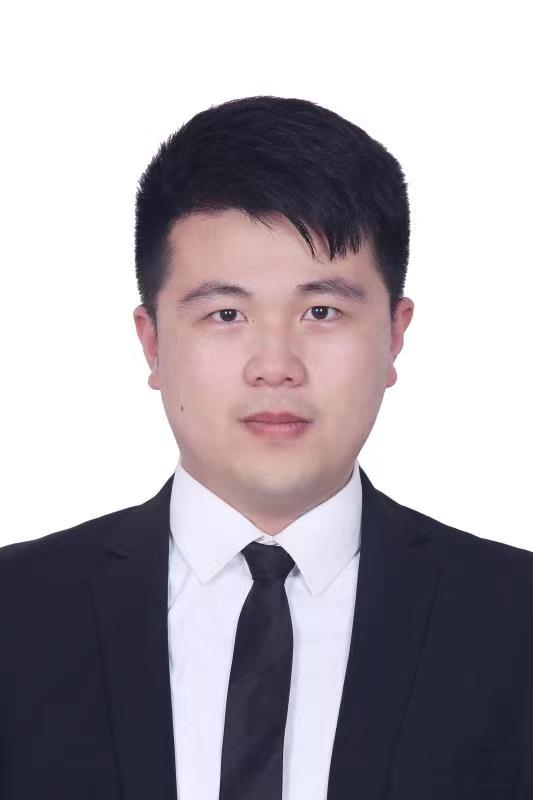
\includegraphics[width=0.9in,height=1.1in,clip,keepaspectratio]{author/Xinyu.jpg}}]{Xinyu Zhang} received the B.E. and the M.S. degree from the Information and Automatic College, Tianjin University of Science and Technology, Tianjin, China, in 2019 and 2022, separately, where he is currently pursuing the Ph.D. degree in intelligent system engineering with Luddy School of Informatics, Computing, and Engineering, Indiana University Bloomington, Bloomington, IN, USA.
His main research includes quantum neural network, deep learning, advanced signal processing, and other disciplines such as information science and large language models (LLMs).
\end{IEEEbiography}


\begin{IEEEbiography}[{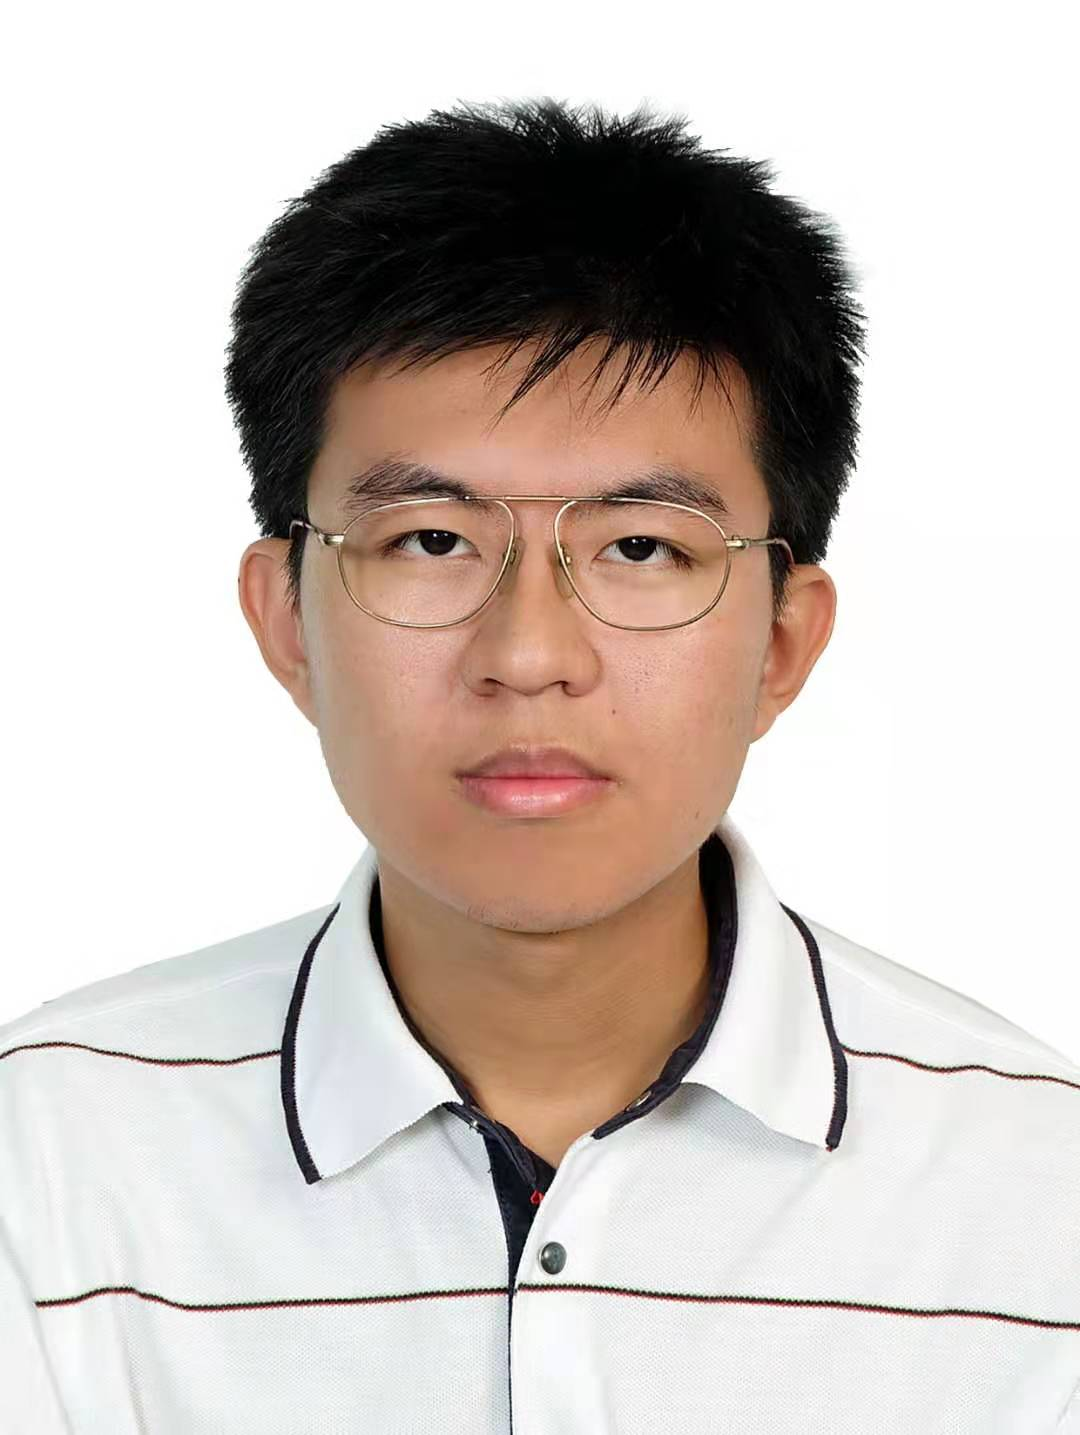
\includegraphics[width=1in,height=1.25in,clip,keepaspectratio]{author/enjui.jpg}}]{En-Jui Kuo}   received the B.S. degree in electrophysics from National Yang Ming University, Taipei, Taiwan. He then obtained his M.S. degree in physics from National Taiwan University, Taipei, Taiwan, and completed his Ph.D. in physics at the University of Maryland, USA. Currently, he is an Assistant Professor of department of electrophysics at the National Yang Ming Chiao Tung University, Taiwan.
\end{IEEEbiography}



\begin{IEEEbiography}[{
\includegraphics[width=0.9in,height=1.1in,clip,keepaspectratio]{author/Rong.jpg}}]{Rong Fu} received the B.S. degree in Communication Engineering from Jiangsu Ocean University, Jiangsu, China, in 2018, and the M.S. degree in Electronic Information Engineering from the College of Information and Automation, Tianjin University of Science and Technology, Tianjin, China, in 2023. She is currently pursuing the Ph.D. degree in Intelligent Systems Engineering with the Luddy School of Informatics, Computing, and Engineering, Indiana University Bloomington, Bloomington, IN, USA. Her research interests include signal processing and deep learning.
\end{IEEEbiography}

\begin{IEEEbiography}[{
\includegraphics[width=0.9in,height=1.1in,clip,keepaspectratio]{author/qiuzhe.jpg}}]{Qiuzhe Xie} received a bachelor's degree in Electrical Engineering from Hefei University of Technology and a master's degree in Electronics Engineering from National Cheng Kung University, followed by a Ph.D. in Electronics Engineering from National Taiwan University. His research expertise encompasses biosensors, advanced semiconductor processes, nanomaterials, and microfabrication techniques. He has spearheaded the development of nano-structural electrode arrays with ultra-thin dielectric stacking and leveraged quantum computing algorithms to enhance sensing precision. Furthermore, he has engineered CRISPR-based electrochemical sensors and developed innovative water purification systems for semiconductor manufacturing. Extending his work to practical application, he also focuses on the commercialization of medical devices, having validated business models for cardiosensor technologies through the NSF program.
\end{IEEEbiography}

\begin{IEEEbiography}[{
\includegraphics[width=0.9in,height=1.1in,clip,keepaspectratio]{author/fan.jpg}}]{Fan Zhang} received the B.S. degree in Statistics from Beijing Normal University, Beijing, China, in 2016, the M.S. degree in statistics from National Cheng Kung University, Taiwan, in 2018, and the Ph.D. degree in statistics from Arizona State University, Tempe, AZ, USA, in 2024. She is currently an Assistant Professor with the Department of Mathematics, Boise State University, Boise, ID, USA. Her research interests include design and analysis of experiments, variable selection, uncertainty quantification, Bayesian modeling and inference, and quantum-enhanced machine learning.

\end{IEEEbiography}


\end{document}
